\documentclass[12pt]{report}

\usepackage[utf8]{inputenc}
%\usepackage[T1]{fontenc}
%\usepackage[français]{babel}
\usepackage{color}
\usepackage[OT1]{fontenc}
\usepackage{lipsum}
\usepackage{graphicx}
\usepackage{geometry}
%--------------------------------------------------------------
%--------------------------------------------------------------
\usepackage{listings}
%\definecolor{darkWhite}{rgb}{0.94,0.94,0.94}
%\definecolor{darkWhite}{rgb}{0.94,0.94,0.94}
\lstset{
	aboveskip=3mm,
	belowskip=-2mm,
	backgroundcolor=\color{white},
	basicstyle=\footnotesize,
	breakatwhitespace=false,
	breaklines=true,
	captionpos=b,
	commentstyle=\color{red},
	deletekeywords={...},
	escapeinside={\%*}{*)},
	extendedchars=true,
	framexleftmargin=16pt,
	framextopmargin=3pt,
	framexbottommargin=6pt,
	frame=tb,
	keepspaces=true,
	keywordstyle=\color{blue},
	language=C,
	literate=
	{²}{{\textsuperscript{2}}}1
	{⁴}{{\textsuperscript{4}}}1
	{⁶}{{\textsuperscript{6}}}1
	{⁸}{{\textsuperscript{8}}}1
	{€}{{\euro{}}}1
	{é}{{\'e}}1
	{è}{{\`{e}}}1
	{ê}{{\^{e}}}1
	{ë}{{\¨{e}}}1
	{É}{{\'{E}}}1
	{Ê}{{\^{E}}}1
	{û}{{\^{u}}}1
	{ù}{{\`{u}}}1
	{â}{{\^{a}}}1
	{à}{{\`{a}}}1
	{á}{{\'{a}}}1
	{ã}{{\~{a}}}1
	{Á}{{\'{A}}}1
	{Â}{{\^{A}}}1
	{Ã}{{\~{A}}}1
	{ç}{{\c{c}}}1
	{Ç}{{\c{C}}}1
	{õ}{{\~{o}}}1
	{ó}{{\'{o}}}1
	{ô}{{\^{o}}}1
	{Õ}{{\~{O}}}1
	{Ó}{{\'{O}}}1
	{Ô}{{\^{O}}}1
	{î}{{\^{i}}}1
	{Î}{{\^{I}}}1
	{í}{{\'{i}}}1
	{Í}{{\~{Í}}}1,
	morekeywords={*,...},
	numbers=left,
	numbersep=10pt,
	numberstyle=\tiny\color{black},
	rulecolor=\color{black},
	showspaces=false,
	showstringspaces=false,
	showtabs=false,
	stepnumber=1,
	stringstyle=\color{cyan},
	tabsize=4,
	title=\lstname,
	basicstyle=\tiny,
}

%------------------------------------------------------------------------------
%------------------------------------------------------------------------------

\geometry{verbose, letterpaper, tmargin=20mm, bmargin=20mm, lmargin=20mm, rmargin=20mm}
%\renewcommand\thechapter{\Roman{chapter}}
\renewcommand\thesection{\Roman{section}}
%\renewcommand\thesubsection{\roman{section}}
\renewcommand\contentsname{\bf \Large \sc Table des Matières}

% \texttt commande comme les 

\begin{document}
	\thispagestyle{empty}
%	\contentsname{KKKK}
	\begin{center}
		\textsc{\large Université d'Abomey-Calavi}             							  		\\ \vspace{3em}  %vfill
		\textsc{\Large Institut de Mathématiques et de Sciences Physiques}                   	\\ \vspace{2em}
		
		
		\rule{0.90\textwidth}{1.67pt}																\\ \vspace{1.2em}

		\textsc{\large Travaux Pratiques Big Data} 	
		
							  		
%		\rule{0.90 \textwidth}{2pt}					
		\vspace{3em}			
		\textsc{\Large Développement d'une Plateforme de Troc d'Objets} 	\\ 
		
		\vspace{2em}
	
		\textsc{Master I - Informatique}
		
			\begin{center}
				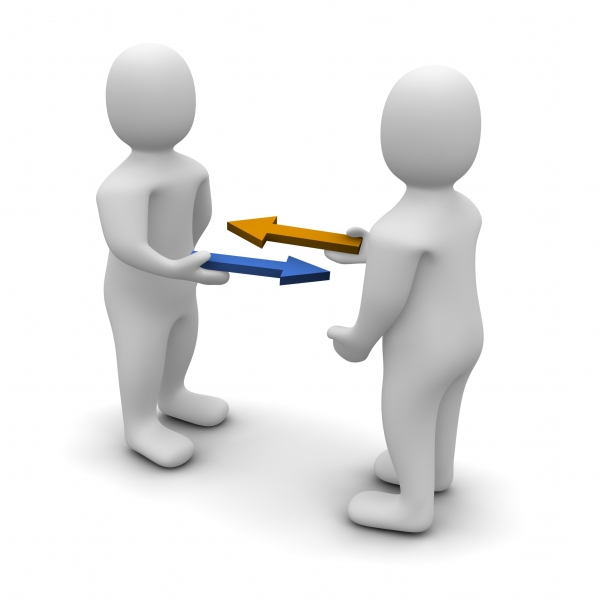
\includegraphics[scale=0.35]{troc4}
				\label{Visual Studio Code}
			\end{center}

		
	
		\vspace{3em}	
		\begin{tabular}{lll}
			\vspace{0.5em}
			 \textsc{\underline{Enseignants:}}	& \hspace{3em}	&	\textsc{\underline{Étudiants:}}		\\ 
			 \textsc{\textbf{\sc Valduriez patrick}} & \hspace{15em}	&	\textsc{\textbf{\sc Gnoguem nestor}}	 \\				%\\ \vspace{1em}
			 \textsc{\textbf{\sc Bondiombouy carlyna}}	& \hspace{15em}	&	\textsc{\textbf{\sc Houngue isaac}}	 \\				%\\ \vspace{1em}
													 	& \hspace{15em}	&	\textsc{\textbf{\sc Saibou aziz}}	 \\				%\\ \vspace{1em}
		\end{tabular}

		\vspace{6.5em}																
%		\fbox{\rule[-0.4cm]{0cm}{1cm} Une boite avec \verb!fbox! et avec \verb!rule!.}
		\textsc{\small Février 2019}
		
		
	\end{center}
	
	\newpage
	\tableofcontents
	
	\newpage

	\section{\sc Introduction générale}
	\rule{1 \textwidth}{0.5pt} \textbf{}
	\vspace{2em}

		\subsection{ \sc Contexte}
		L’explosion quantitative des données numériques a obligé les chercheurs à trouver de nouvelles
		manières de voir et d’analyser le monde. Il s’agit en effet de découvrir de nouveaux ordres de
		grandeur concernant la capture, la recherche, le partage, le stockage, l’analyse et la présentation des données. Ainsi est né le \texttt{Big Data}. Il s’agit d’un concept permettant de stocker un nombre indicible d’informations sur une base numérique. Littéralement, le \texttt{Big Data} signifie les mégadonnées, grosses données ou encore données massives.
		Ils désignent un ensemble très volumineux de données qu’aucun outil classique de gestion de base
		de données ou de gestion de l’information ne peut vraiment travailler.
		En effet, nous procréons environ 2,5 trillions d’octets de données tous les jours. Ce sont les informations provenant de partout (les message que nous nous envoyés, les vidéos que nous publions, les informations climatiques, les signaux {\sc gps}, les enregistrements transactionnels d’achats en ligne et bien
		d’autres encore).

		\subsection{ \sc Problématique}
	Il n'est pas évident de reconnaître la nécessité ou non de l'utilisation des technologies du \texttt{Big Data} dans les projets informatiques. Il est donc utile de pratiquer (expérimenter) afin d'acquérir de l'expérience en ce qui concerne le choix des outils ou technologies du \texttt{Big Data}. Le projet qu'on s'est fait attribuer portant sur la \texttt{Plateforme troc} nous permettra de mettre en \oe uvre nos connaissance sur les concepts.
		\subsection{ \sc Objectifs}
		Notre projet permettra à toute personne de trouver des avec qui troquer librement ses produits. On doit tout de même rendre compte de la compréhension du dataset de la definition du metier, technique, besoin en données, de cas d'utilisation de notre application qui ne sont rien d'autre que les fonctionnalités de notre application. On doit également rendre compte de la maîtrise des outils suivants: \texttt{HDFS
			, Spark , Spark , Neo4J , MongoDB.} 
		
		\subsection{ \sc Plan du rapport}
		Partant de l'analyse et à la réalisation, on exposera toutes les différentes étapes nécessaires à la construction de notre programme. Il suivra donc une conclusion résumant tout notre travail.
%		\rule{0.7 \textwidth}{2pt} \textbf{}

	\newpage
	 \section{\sc Description du projet}
	 \rule{1 \textwidth}{0.5pt} \textbf{}
	 
	 \vspace{2em}
	 Un client dans un processus dans un processus de troc a la possibilité de visualiser tous ces produits en cours de troc et le produit à troquer
	 Par soucis d'économie, désir de solidarité, ou encore pour trouver la perle rare on peut échanger des objets(vêtements, voitures, livres, etc..). C'est le système de troc sur internet. En effet intervient entre deux ou plusieurs individus ayant des objets à échanger. Dès que l'individu. Lorsque la partie 1 poste un objet, la seconde partie a la possibilité d'accepter ou non afin de valider l'effectivités de l'opération. Le site s'occupe lui même de l'envoi ou fournit des netiquettes à aposer sur les objets. Mais les troqueurs parfois choisissent de s'arranger entre eux en s'expédiant des objets par courrier ou en se donnant de rendez-vous, d'ou la formule d'abonnement. Le 
	 
	 xxxxxxxxxxxxxxxxxxxxxxxxxxxxxxxxxxxxxxxxxxxxxxxxxxxxxxxxxxxxxxxxxxx
	 
	 xxxxxxxxxxxxxxxxxxxxxxxxxxxxxxxxxxxxxxxxxxxxxxxxxxxxxxxxxxxxxxxxxxx
	 
	 xxxxxxxxxxxxxxxxxxxxxxxxxxxxxxxxxxxxxxxxxxxxxxxxxxxxxxxxxxxxxxxxxxx
	 
	 xxxxxxxxxxxxxxxxxxxxxxxxxxxxxxxxxxxxxxxxxxxxxxxxxxxxxxxxxxxxxxxxxxx
	 
	  xxxxxxxxxxxxxxxxxxxxxxxxxxxxxxxxxxxxxxxxxxxxxxxxxxxxxxxxxxxxxxxxxxx
	  
	  xxxxxxxxxxxxxxxxxxxxxxxxxxxxxxxxxxxxxxxxxxxxxxxxxxxxxxxxxxxxxxxxxxx
	  
	  xxxxxxxxxxxxxxxxxxxxxxxxxxxxxxxxxxxxxxxxxxxxxxxxxxxxxxxxxxxxxxxxxxx
	  
	  xxxxxxxxxxxxxxxxxxxxxxxxxxxxxxxxxxxxxxxxxxxxxxxxxxxxxxxxxxxxxxxxxxx

	\newpage
	\section{\sc Analyse et Conception}
		\rule{1 \textwidth}{0.5pt} \textbf{}
		
		\vspace{2em}
		L’analyse des besoins est une phase qui consiste à comprendre et à déterminer
		les différentes fonctionnalités et besoins du système.
		L'identification des acteurs d'une application est une phase primordial de l'analyse des besoins c'est ainsi qu'on a pu identifier les acteurs suivants:
		\begin{description}
			\item [\sc Client:] Toute personne physique capable de poster ou de consulter un objet.
			\item[\sc Administrateur:] Toute personne susceptible de maintenir le système du point de vue gestion des compte des utilisateurs.
		\end{description}
		 Les besoins fonctionnels constituent les fonctionnalités que le système devra assurer, parmi les
		 quelles, nous décrivons principalement les fonctions suivantes: 
		 \begin{enumerate}
		 	\item Consulter des objets
		 	\item Troquer un objet
		 	\item Ajouter un objet
		 \end{enumerate}
		 Le diagramme des cas d'utilisation suivant rend compte des fonctionnalités de notre application
			\begin{center}
				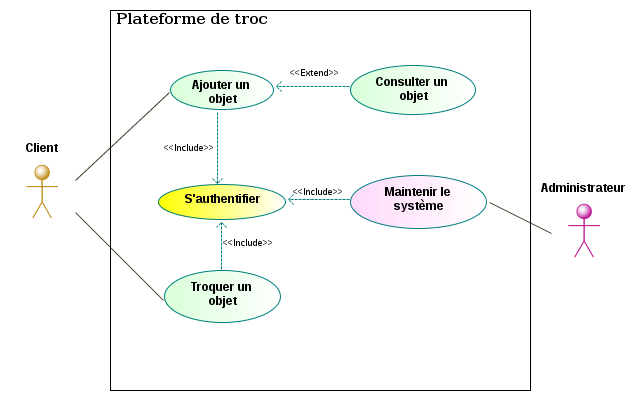
\includegraphics[scale=1, width=\textwidth, height=10cm]{usecase}
				\label{usecase}
			\end{center}
			
			Après la description des différents cas d’utilisation, nous allons élaborer le modèle dynamique
			dans lequel nous allons décrire les scénarios de quelques cas d’utilisations les plus importants sous forme de diagrammes de séquence.
			
			\begin{center}
				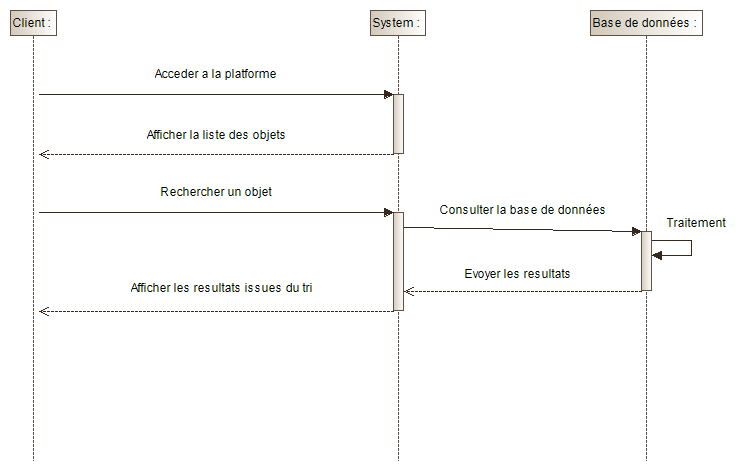
\includegraphics[scale=1, width=0.8\textwidth, height=10cm]{troc0}
				\label{troc0}
			\end{center}
			\begin{center}
				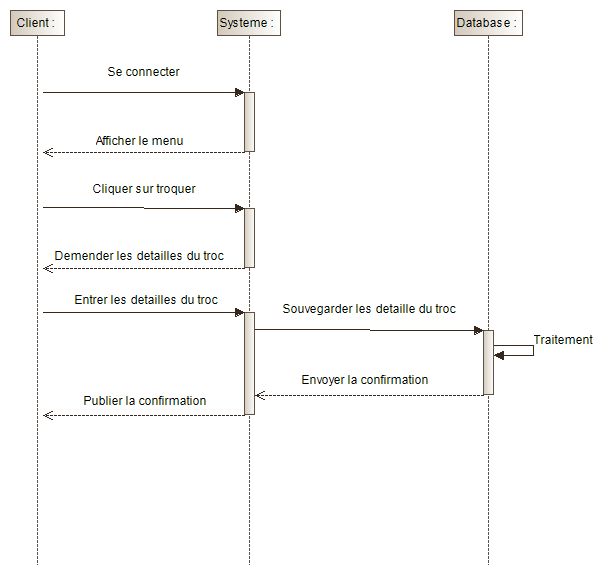
\includegraphics[scale=1, width=0.8\textwidth, height=10cm]{troc1}
				\label{troc1}
			\end{center}
	Le diagramme de classe dictant le comportement de notre programme est le suivant:
		 	\begin{center}
		 		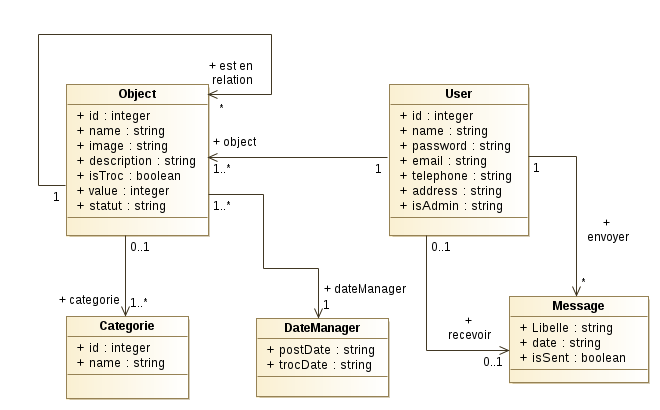
\includegraphics[scale=1, width=0.9\textwidth, height=10cm]{class}
		 		\label{class}
		 	\end{center}
	
	 
	
	 
	 
	\newpage
	\section{\sc Réalisation}
		\rule{1 \textwidth}{0.5pt} \textbf{}
		\vspace{2em}
	
	\subsection{\sc Environnement de développement logiciel}
	
	
	\subsubsection{\sc Choix de la base du sgbd NoSQL}
	
	En vue d'écrire un programme cohérent et consistant nous avons adopté la structuration suivante pour nos  fichiers.
	
	xxxxxxxxxxxxxxxxxxxxxxxxxxxx
	xxxxxxxxxxxxxxxxxxxxxxxxxxxx
	
{\flushleft	Les outils logiciels que nous avons utilisé sont les suivants:}
	\begin{description}
		\item[\sc Modelio 3.7:] Un logiciel de modélisation open-source
				\begin{center}
					
\includegraphics[scale=1, width=0.56\textwidth, height=4cm]{modelio}
					\label{modelio}
				\end{center}
		
		\item[\sc Visual-Studio-Code 1.28:] Un éditeur de texte avancé
				\begin{center}
					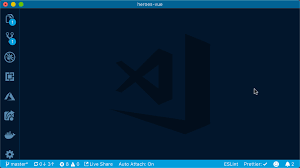
\includegraphics[scale=1, width=0.5\textwidth, height=5cm]{vscode}
					\label{vscode}
				\end{center}
		\item[\sc Flask 1.0:]  Un \textit{mini-framework} open-source de développement web en Python
		
				\begin{center}
					
\includegraphics[scale=1, width=0.5\textwidth, height=4cm]{flask}
					\label{flask}
				\end{center}
		\item[\sc Jinja2:] Un moteur de template
			\begin{center}
				
\includegraphics[scale=1, width=0.5\textwidth, height=4cm]{jinja}
				\label{jinja}
			\end{center}
			
		\item[\sc Mongo-DB:] Un système de gestion de base de données orienté document open-source developpé en {\tt C++}
			\begin{center}
				
\includegraphics[scale=1, width=0.5\textwidth, height=4cm]{mongo}
				\label{mongo}
			\end{center}
			
		
			
	\end{description}
	
	\subsection{\sc Démonstration}
	
	

	\newpage
	\section{\sc Conclusion}
		\rule{1 \textwidth}{0.5pt} \textbf{}
		\vspace{2em}
		
		La théorie des est une branche des mathématiques amenant le besoin de classifier les problèmes courants. C'est ainsi que cette théorie offre beaucoup de moyens ou pistes pour la résolution de problèmes. L'étude de la théorie des graphes à améliorer notre manière de raisonner, sans oublier que les algorithmes implémentés dans ce projet non seulement nous ont aidé à comprendre le cours mais aussi à approfondir notre connaissance en programmation.
\end{document}